\gls{dqn} is a reinforcement learning algorithm that combines Q-learning
with deep learning. The algorithm uses a neural network to approximate the
Q-values of the state-action pairs. The Q-values are updated using the Bellman
equation, which is defined as follows:
\begin{equation}
    Q(S_t, A_t) \leftarrow Q(S_t, A_t) + \alpha [R_{t+1} + \gamma \max_{a} Q(S_{t+1}, a) - Q(S_t, A_t)]
\end{equation}

The \hyperref[alg:dqn]{algorithm} uses experience replay to store and sample
transitions from the environment. The transitions are stored in a replay
memory, which is a fixed-size buffer. The algorithm samples a random minibatch
of transitions from the replay memory to update the Q-values. This helps to
break the correlation between the samples and stabilize the training process.

\begin{algorithm}[H]
    \begin{algorithmic}[1]
        \State Initialize replay memory $D$ to capacity $N$
        \State Initialize action-value function $Q$ with random weights $\theta$
        \For{episode $= 1, M$}
            \State Initialize sequence $s_1 = \{x_1\}$ and preprocessed sequence $\phi_1 = \phi(s_1)$
            \For{t $= 1, T$}
                \State With probability $\epsilon$ select a random action $a_t$
                \State otherwise select $a_t = \argmax_a Q(\phi(s_t), a; \theta)$
                \State Execute action $a_t$ in emulator and observe reward $r_t$ and image $x_{t+1}$
                \State Set $s_{t+1} = s_t, a_t, x_{t+1}$ and preprocess $\phi_{t+1} = \phi(s_{t+1})$
                \State Store transition $(\phi_t, a_t, r_t, \phi_{t+1})$ in $D$
                \State Sample random minibatch of transitions $(\phi_j, a_j, r_j, \phi_{j+1})$ from $D$
                \State Set $y_j = \begin{cases}
                    r_j & \text{if episode terminates at step } j+1 \\
                    r_j + \gamma \max_{a^\prime} Q(\phi_{j+1}, a^\prime; \theta) & \text{otherwise}
                \end{cases}$
                \State Perform a gradient descent step on $(y_j - Q(\phi_j, a_j; \theta))^2$ with respect to the network parameters $\theta$
            \EndFor
        \EndFor
    \end{algorithmic}
    \caption{Deep Q-learning}
    \label{alg:dqn}
\end{algorithm}

\subsection{Double Deep Q-learning}\label{sec:agent-dqn-ddqn}
Much like \gls{dqn}, \gls{ddqn} is a reinforcement learning algorithm that
combines Q-learning with deep learning. The algorithm uses a neural network to
approximate the Q-values of the state-action pairs, and also updates the
Q-values using the Bellman equation, which is defined as follows:
\begin{equation}
    Q(S_t, A_t) \leftarrow Q(S_t, A_t) + \alpha [R_{t+1} + \gamma \max_{a} \hat{Q}(S_{t+1}, a) - Q(S_t, A_t)]    
\end{equation}

The key difference between \gls{dqn} and \gls{ddqn} is that the Q-values are
updated using the maximum Q-value of the next state according to the target
action-value function. This helps to reduce the overestimation of the Q-values
and improve the stability of the training process. This target action-value
function is referred to as $\hat{Q}$, and is updated every $C$ steps to match
the action-value function $Q$. Like \gls{dqn} \hyperref[alg:ddqn]{algorithm}
uses experience replay.

\begin{algorithm}[H]
    \begin{algorithmic}[1]
        \State Initialize replay memory $D$ to capacity $N$
        \State Initialize action-value function $Q$ with random weights $\theta$
        \State Initialize target action-value function $\hat{Q}$ with weights $\theta^- = \theta$
        \For{episode $= 1, M$}
            \State Initialize sequence $s_1 = \{x_1\}$ and preprocessed sequence $\phi_1 = \phi(s_1)$
            \For{t $= 1, T$}
                \State With probability $\epsilon$ select a random action $a_t$
                \State otherwise select $a_t = \argmax_a Q(\phi(s_t), a; \theta)$
                \State Execute action $a_t$ in emulator and observe reward $r_t$ and image $x_{t+1}$
                \State Set $s_{t+1} = s_t, a_t, x_{t+1}$ and preprocess $\phi_{t+1} = \phi(s_{t+1})$
                \State Store transition $(\phi_t, a_t, r_t, \phi_{t+1})$ in $D$
                \State Sample random minibatch of transitions $(\phi_j, a_j, r_j, \phi_{j+1})$ from $D$
                \State Set $y_j = \begin{cases}
                    r_j & \text{if episode terminates at step } j+1 \\
                    r_j + \gamma \max_{a^\prime} \hat{Q}(\phi_{j+1}, a^\prime; \theta^-) & \text{otherwise}
                \end{cases}$
                \State Perform a gradient descent step on $(y_j - Q(\phi_j, a_j; \theta))^2$ with respect to the network parameters $\theta$
                \State Every $C$ steps reset $\hat{Q} = Q$
            \EndFor
        \EndFor
    \end{algorithmic}
    \caption{Double Deep Q-learning}
    \label{alg:ddqn}
\end{algorithm}

\subsection{Prioritized Experience Replay}\label{sec:agent-dqn-per}
\subsubsection{Importance Sampling}\label{sec:agent-dqn-per-importance-sampling}
Importance sampling is a technique used to estimate the expected value of
a function under a different distribution. In the context of reinforcement
learning, importance sampling is used to estimate the expected value of the
Q-values under the target policy, given that the Q-values are estimated under
the behavior policy. This is useful when the target policy is different from
the behavior policy, as it allows the agent to learn how to act optimally under
the target policy.

In the context of the \gls{per} algorithm, importance sampling is used to
correct the bias introduced by the prioritized replay. The bias is caused by
the fact that the priorities are updated frequently, which can lead to
overestimation of the Q-values. To correct this bias, the \gls{per} algorithm
uses importance sampling to reweight the updates to the Q-values based on the
importance of the transitions. This helps to reduce the bias and improve the
stability of the learning process.

The importance sampling weight is calculated as follows:
\begin{equation}
    w_i = \left( \frac{1}{N} \cdot \frac{1}{P(i)} \right)^{\beta}
\end{equation}

\subsection{Results}\label{sec:agent-dqn-results}
Our initial results are from our own implementation of \gls{ddqn} with
a learning rate of 0.001, a discount factor of 0.99, and a batch size of 32.
The neural netowrk has two hidden layers with 1024 units each and uses the
ReLU activation function. The target network is updated every 1000 steps,
and prioritized experience replay is used with $\alpha = 0.6$ and
$\beta = 0.4$.

\begin{figure}[H]
    \begin{subfigure}{0.45\textwidth}
        \centering
        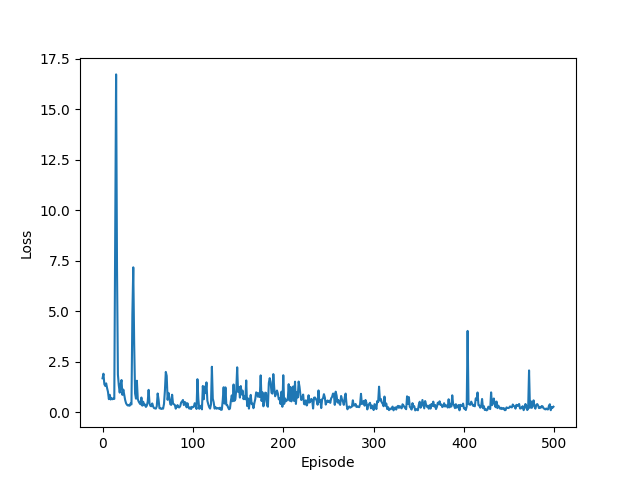
\includegraphics[width=\textwidth]{img/ddqn-500-loss.png}
        \caption{Loss over 500 episodes}
        \label{fig:ddqn-500-loss}
    \end{subfigure}
    \begin{subfigure}{0.45\textwidth}
        \centering
        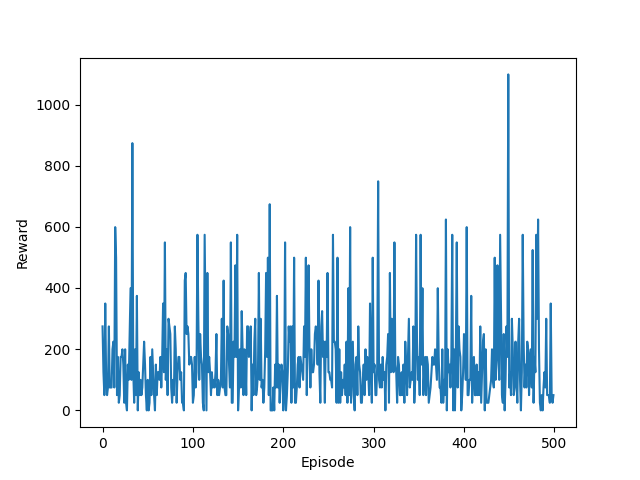
\includegraphics[width=\textwidth]{img/ddqn-500-reward.png}
        \caption{Reward over 500 episodes}
        \label{fig:ddqn-500-reward}
    \end{subfigure}
    \caption{Double DQN training results}
    \label{fig:ddqn-500}
\end{figure}

As we can see in \cref{fig:ddqn-500}, the loss converges to a value of
approximately 0.5, but the reward does not seem to improve significantly.
This is also confirmed through testing, where the agent simply seems to move
to the left, jumping off and dying. This could be due to several reasons,
all of which mentioned previously in \cref{ch:environment}.

Training the agent for 1600 episodes, we see a similar pattern, followed
by a very unusual spike in the loss, as seen in \cref{fig:ddqn-2000-1600-loss}.

\begin{figure}[H]
    \begin{subfigure}{0.45\textwidth}
        \centering
        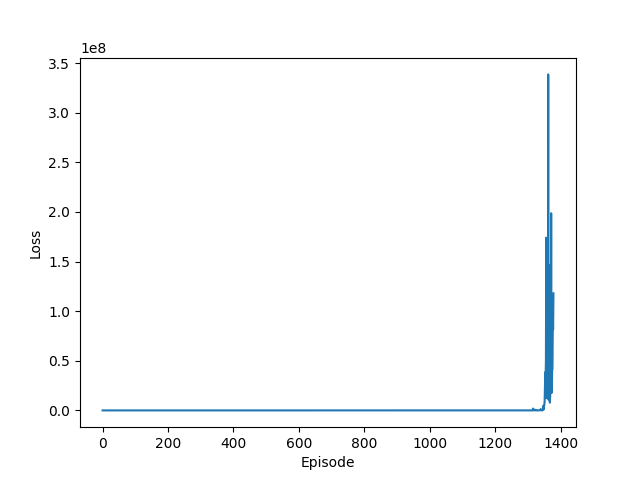
\includegraphics[width=\textwidth]{img/ddqn-2000-1600-loss.png}
        \caption{Loss over 1600 episodes}
        \label{fig:ddqn-2000-1600-loss}
    \end{subfigure}
    \begin{subfigure}{0.45\textwidth}
        \centering
        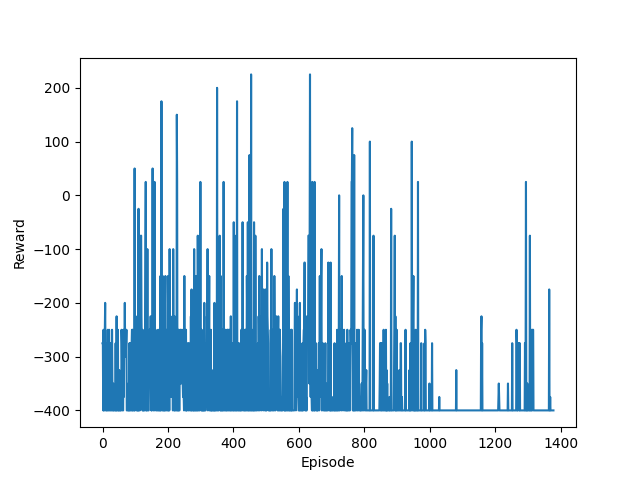
\includegraphics[width=\textwidth]{img/ddqn-2000-1600-reward.png}
        \caption{Reward over 1600 episodes}
        \label{fig:ddqn-2000-1600-reward}
    \end{subfigure}
    \caption{Double DQN training results}
    \label{fig:ddqn-2000-1600}
\end{figure}

Here, we see that the loss remains low, but then suddenly increases into the
billions. This is likely due to the Q-values exploding, which is a common
problem in \gls{rl} algorithms. We can combat this by using gradient clipping,
which limits the size of the gradients, or by using a different architecture
for the neural network.

Another point to consider is the training speed. Even with a strong GPU, the
training process is very slow, and it is difficult to experiment with different
hyperparameters. This is why we have chosen to use Stabe Baselines 3, which
provides a more efficient implementation of the algorithms.

Using the a learning rate of 0.0001, and having implemented all of the
improvements mentioned in \cref{ch:environment}, we trained a \gls{dqn} agent
for 40 million steps. The results can be seen in \cref{fig:dqn}.

\begin{figure}[H]
    \begin{subfigure}{0.45\textwidth}
        \centering
        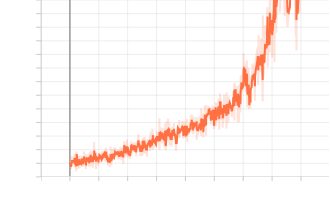
\includegraphics[width=\textwidth]{img/dqn_len_mean.png}
        \caption{Mean episode length}
        \label{fig:dqn_len_mean}
    \end{subfigure}
    \begin{subfigure}{0.45\textwidth}
        \centering
        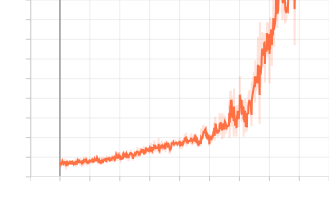
\includegraphics[width=\textwidth]{img/dqn_rew_mean.png}
        \caption{Mean episode reward}
        \label{fig:dqn_reward_mean}
    \end{subfigure}
    \caption{DQN training results}
    \label{fig:dqn}
\end{figure}

As we can see in \cref{fig:dqn}, the agent is able to learn to play the game
quite well, with the mean episode length and the mean episode reward increasing 
steadily. Also through testing, the agent is able to complete several levels
of the game, which is a significant improvement over the previous results.

However, the agent still has some issues. It is not able to complete the game
consistently, and it still has a tendency to jump off the platform and die.
This could be due to the fact that the agent is not able to learn the optimal
policy, or that the environment is too complex for the agent to learn. It could
also be due to the factors surrounding the number of lives mentioned in
\cref{sec:environment-termination}.

Although it may be interesting to continue training the agent, we have chosen
to move on to the next algorithm, \gls{ppo}, as it is more efficient and
provides better results in general.
